\chapter{Time-independent Schrodinger equation}
\section{Stationary states}
Wa talked a lot about the wave function, and how you use it to calculare various quantities of interest. But, how do get $\Psi(x,t)$ in the first place? We need to solce the Schrodinger equation,
\begin{equation}\label{2.1}
	i\hbar\pdv{\Psi}{t}=-\frac{\hbar^2}{2m}\pdv[2]{\Psi}{x}+V\Psi
\end{equation}
for a specified potential\footnote{It is tiresome to keep saying "potential energy function", so most people jus call $V$ the "potential", even though this invites occasional confusion with electric potencial, which is actually potential energy per unit charge.} $V(x,t)$. In this chapter (and most of this book) I shall assume that $V$ is \textit{independent} of $t$. In that case the Schrodinger equation can be solved by the method of \textbf{separation of variables}: We look for solutions that are simple \textit{products},
\begin{equation}\label{2.2}
	\Psi(x,t)=\psi(x)\varphi(t)
\end{equation}
where $\psi$ is a function of $x$ alone, and $\varphi$ is a function of $t$ alone. 

For separable solutions we have
\begin{equation*}
	\pdv{\Psi}{t}=\psi\dv{\varphi}{t},\qquad \pdv[2]{\Psi}{x}=\dv[2]{\psi}{x}\varphi
\end{equation*}
(\textit{ordinaty} derivatives, now), and Schrodinger equation reads
\begin{equation}
	i\hbar\dv{\varphi}{t}=-\frac{\hbar^2}{2m}\dv[2]{\psi}{x}\varphi + V\psi\varphi
\end{equation}
Or, dividing through by $\psi\varphi$:
\begin{equation}\label{2.3}
	i\hbar\frac{1}{\varphi}\dv{\varphi}{t}=-\frac{\hbar^2}{2m}\frac{1}{\psi}\dv[2]{\psi}{x}+V
\end{equation}

Now, the left side is a function of $t$ alone, and the right side is a function of $x$ alone\footnote{Note that this would not be true if $V$ were a function of $t$ as well as $x$.}. The only way this can possibly be true is if both sides are in fact \textit{constant} -- otherwise, by varying $t$, I could change the left side without touching the right side, and the two would no lonegr equal. For reasons that will appear in a moment, we shall call the separation constan $E$. Then
\begin{equation*}
	i\hbar\frac{1}{\varphi}\dv{\varphi}{t}=E
\end{equation*}
or
\begin{equation*}\label{2.4}
	\dv{\varphi}{t}=-\frac{iE}{\hbar}\varphi
\end{equation*}
and
\begin{equation}
	-\frac{\hbar^2}{2m}\frac{1}{\psi}\dv[2]{\psi}{x}+V=E
\end{equation}
or
\begin{equation}\label{2.5}\marginnote{Time-independent Schrodinger equation}
	\boxed{-\frac{\hbar^2}{2m}\dv[2]{\psi}{x}+V\psi=E\psi}
\end{equation}
Separation of variables hs turned a \textit{partial} differential equation into \textit{two ordinary} differential equations (\ref{2.4}) and (\ref{2.5}). The first, (\ref{2.4}) is easy to solve (just multiply through by $\dd t$ and integrate); the general solution is $C\exp(-iEt/\hbar)$, but we might as well absorb the constant $C$ into $\psi$ (since the quantity of interest is the product $\psi\varphi$). Then
\begin{equation}\label{2.6}
	\varphi(t)=e^{-iEt/\hbar}
\end{equation}
The second equation (\ref{2.5}) is called the \textit{time-independent Schrodinger equation} we can go further with it until the potencial $V(x)$ is specified.

The rest of thus chapter will be devoted to solving the time-independent Schrodinger equation, fot a variety of simple potentials. But before I get to that you have every right ask: What's so great about separable solutions? After all, most solutions so the (time dependent) Schrodinger equation do not take the form $\psi(x)\varphi(t)$. I offer three answers--two of them physical, and one mathematical:
\begin{enumerate}
	\item They are \textbf{stationaty states}. Although the wave function itself,
		\begin{equation}\label{2.7}
	\Psi(x,t)=\psi(x)e^{-iEt/\hbar}
\end{equation}
does (obviously) depende on $t$, the \textit{probability density},
\begin{equation}\label{2.8}
	|\Psi(x,t)|^2=\Psi^*\Psi=\psi^*e^{+iEt/\hbar}\psi e^{-iEt/\hbar}=|\psi(x)|^2
\end{equation}
does not--the time-dependence cancels out\footnote{For normalizable solutions, $E$ must be real}. The same thing happens in calculate the expectation value of any dynamil variable; (\ref{1.36}) reduces to
\begin{equation}\label{2.9}
	<Q(x,p)>=\int\psi^*Q\left(x,\frac{\hbar}{i}\frac{\dd}{\dd x}\right)\psi\dd x
\end{equation}
\textit{Every expectation value is constant in time}; we might as well drop the factor $\varphi(t)$ altogether, and simply use $\psi$ in place of $\Psi$. In particular, $<x>$ is constant, and hence $<p>=0$ (See (\ref{1.33})). Nothing ever happens in a stationary state.

\item They are states of \textit{definite total energy}. In classical mechanics, the total energy (kinetic plus pontential) is called the \textbf{Hamiltonian}:
	\begin{equation}\label{2.10}
	H(x,p)=\frac{p^2}{2m}+V(x)
\end{equation}
The corresponding Hamiltonian \textit{operator}, obtained by the canonical substitution $p\to (\hbar/i)(\partial /\partial x)$, is therefore\footnote{Whenever confusion might arise. I'll put a "hat" on the operator, to distinguish it from the dynamical variable it represents.}
\begin{equation}\label{2.11}
	\hat{H}=-\frac{\hbar^2}{2m}\frac{\partial^2}{\partial x^2}+V(x)
\end{equation}
Thus the time-independent Schrodinger equation (\ref{2.5}) can be written
\begin{equation}\label{2.12}
	\hat{H}\psi=E\psi
\end{equation}
and the expectation value of the total energy is
\begin{equation}\label{2.13}
	<H>=\int\psi^*\hat{H}\psi\dd x=E\int |\psi|^2\dd x=E\int |\Psi|^2\dd x=E
\end{equation}
(Notice that the normalization of $\Psi$ entails the normalization of $\psi$.) Moreover,
$$\hat{H}^2\psi=\hat{H}(\hat{H}\psi)=\hat{H}(E\psi)=E(\hat{H}\psi)=E^2\psi$$ and hence $$<H^2>=\int\psi^*\hat{H}^2\psi\dd x=E^2\int|\psi|^2\dd x=E^2$$ So the variance of $H$ is 
\begin{equation}\label{2.14}
	\sigma_H^2=<H^2>-<H>^2=E^2-E^2=0
\end{equation}
But remember, if $\sigma=0$, then every member of the sample must share the same value (the distribution has zero spread). \textit{Conclusion}: A separable solution has the property that \textit{every measurement of the total energy is certain to return the value $E$}.

\item The general solution is a \textbf{linear combiantion} of separable solutions. As we're about to discover, the time-independent Schrodinger equation (\ref{2.5}) yields an infinite collection of solution ($\psi_1(x), \psi_2(x),...$),  each with its assocaites value of the reparation constant ($E_1, E_2, ...$); thus there is a different wave function for each \textbf{allowed energy}:
	$$\Psi_1(x,t)=\psi_1(x)e^{-iE_1t/\hbar},\qquad \Psi_2(x,t)=\psi_2(x)e^{-iE_2t/\hbar}, ...$$ Nowthe time-dependent Schrodinger equation (\ref{2.1}) has the property that any linear combination\footnote{A \textbf{linear combination} of the functions $f_1(z), f_z(z),...$ is an expression of the form $$f(z)=c_1f_1(z)+c_2f_2(z)+\cdots$$ where $c_1,c_2,...$ are any (complex) constants.} of solutions is itself a solution. Once we have found the separable solutions, then, we can immediately construct a much more general solution, on the form
	\begin{equation}\label{2.15}
	\Psi(x,t)=\sum_{n=1}^\infty c_n\psi_n(x)e^{-iE_nt/\hbar}
\end{equation}
It so happens that \textit{every} solution to the (time-dependent) Schrodinger equation can be written iun this form --it is simply a matter if finding the tight constants ($c_1,c_2,...$) so as to fit the initial conditions for the problem at hand.

Let me recapitulate, from a somewhat different persperctive. Here's the generic problem: You're given a (time-independent) potencial $V(x)$ and the starting wave function $\Psi(x,0)$; your job is to find the wave function, $\Psi(x,t)$, for any subsequent time $t$. To do this you must solve the (time-dependent) Schrodinger equation (\ref{2.1}); this yields, in general, an infinite set of solutions ($\psi_1(x),\psi_2(x),...$), each with its own assocaited energy ($E_1,E_2,...$). To fit $\Psi(x,0)$ you write down the general linear combination of these solutions:
\begin{equation}\label{2.16}
	\Psi(x,0)=\sum_{n=1}^\infty c_n\psi_n(x)
\end{equation}
the miraacle os that you can \textit{always} match the specified initial state by appropiate choice of the constants $c_1,c_2,...$. To construct $\Psi(x,t)$ you simply tack onto each term its characteristic time dependence, $\exp(-iE_nt/\hbar)$:
\begin{equation}\label{2.17}
	\boxed{\Psi(x,t)=\sum_{n=1}^\infty c_n\psi_n(x)e^{-iE_nt/\hbar}=\sum_{n=1}^\infty c_n\Psi_n(x,t)}
\end{equation}
The separable solutions themselves,
\begin{equation}\label{2.18}
	\Psi_n(x,t)=\psi_n(x)e^{-iE_nt/\hbar}
\end{equation}
are \textit{stationary} states, in the sense that all probabilities and expectation values are independent of time, but this property is emphatically \textit{not} shared by the general solution (\ref{2.17}); the enrgies are different, for different stationary states, and the exponentials do not cancel, when you calculate $|\Psi|^2$.

\section{The infinite square well}
\begin{figure}[h!]
	\begin{center}
		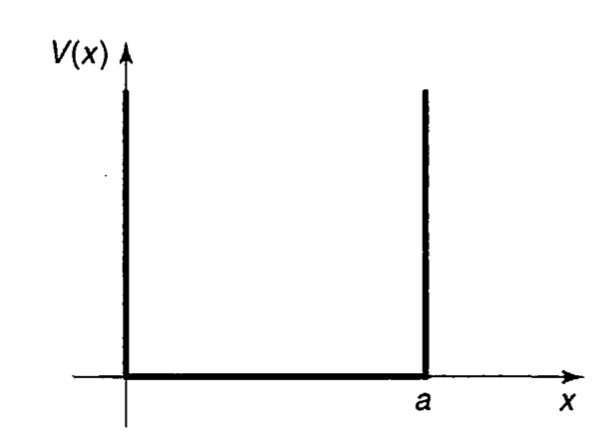
\includegraphics[scale=0.5]{fig/01.png}
		\caption{The infinte square well potential (\ref{2.19})}
		\label{fig:2.1}
	\end{center}	
\end{figure}

Suppose
\begin{equation}\label{2.19}
	V(x)=\left\{\begin{array}{lc}
		0&,0\leq x\leq a\\ \infty & \mbox{,otherwise}\end{array}
		\right.
\end{equation}
Fig. (\ref{fig:2.1}). A particle in this potential is completely free, except at two ends ($x=0$ and $x=a$), where an infinte force prevents it from escaping.

\textit{Outside} the well, $\psi(x)=0$ (the probability of findig the particle there is zero) \textit{Inside} the well, where $V=0$, the time-independent Schrodinger equation (\ref{2.5}) reads
\begin{equation}\label{2.20}
	-\frac{\hbar^2}{2m}\dv[2]{\psi}{x}=E\psi
\end{equation}
or
\begin{equation}\label{2.21}
	\dv[2]{\psi}{x}=-k^2\psi,\qquad \mbox{where } k\equiv\frac{\sqrt{2mE}}{\hbar}
\end{equation}
(By writinf it in this way, I have tacitly assumed that $E\geq 0$.) Equation (\ref{2.21}) is the classical \textbf{simple harmonic oscilaltor} equation; the general solution is
\begin{equation}\label{2.22}
	\psi(x)=A\sin kx + B\cos kx
\end{equation}
where $A$ and $B$ are arbitraty constants. Tipically, these constants are fixed by the \textbf{boundary conditions} of the problem. What are the appropiate boundary conditions for $\psi(x)$? Ordinatily, both $\psi$ and $\dd \psi/\dd x$ are continuous, but where the potential goes to infinity only the first of these applies.

Continuity of $\psi(x)$ requieres that
\begin{equation}\label{2.23}
	\psi(0)=\psi(a)=0
\end{equation}
so as to join onto the solution outisde the well. What does this tell us about $A$ and $B$? Well,
\begin{equation*}
	\psi(0)=A\sin 0+B\cos 0=B
\end{equation*}
so $B=0$, and hence
\begin{equation}\label{2.24}
	\psi(x)=A\sin kx
\end{equation}
Then $\psi(a)=A\sin ka$, so either $A=0$ (in which case we're left with the trivial --non-normalizable--solution $\psi(x)=0$), or else $\sin ka=0$, which means that
\begin{equation}\label{2.25}
	ka = 0,\pm \pi,\pm 2\pi,\pm 3\pi,...
\end{equation}
But $k=0$ is no good (again, that would imply $\psi(x)=0$),and the negative solutions give nothing new, since $\sin(-\theta)=-\sin(\theta)$ andw e can absorb the minus sign into $A$. So the \textit{distinct} solutions are
\begin{equation}\label{2.26}
	k_n=\frac{n\pi}{a},\qquad \mbox{with } n=1,2,3,...
\end{equation}
Curiously, the boundary condition at $x=a$ does not determine the constant $A$, but rather the constant $k$, and hence the possible values of $E$:
\begin{equation}\label{2.27}\marginnote{Possible values of $E$}
	\boxed{E_n=\frac{\hbar^2k_n^2}{2m}=\frac{n^2\pi^2\hbar^2}{2ma^2}}
\end{equation}










\end{enumerate}



